\section{Preliminaries}
\label{sec:perliminary}

\begin{figure}[tbp]
	\hspace{0ex}
	\vspace{0ex}
	\centering
	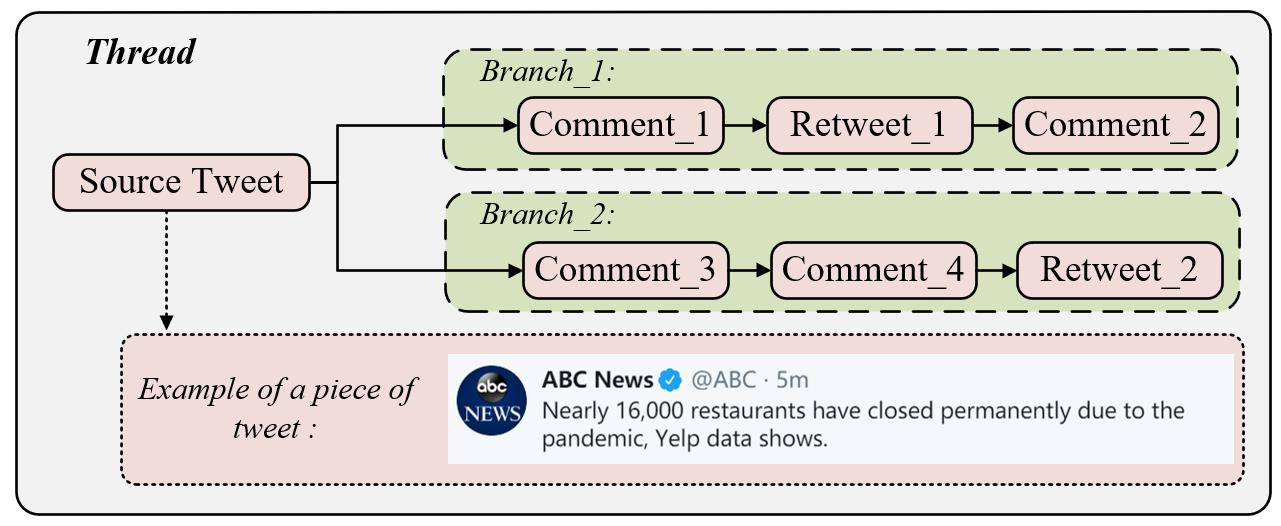
\includegraphics[width = \textwidth]{fig/data_format}
	\caption{The data format of a tweet thread}
	\label{fig:data_format}
\end{figure}

In this section, we proceed to introduce the notations, problem definitions, and background knowledge of rumor tracking. The frequently used notations are summarized in Table~\ref{tab:notations}.

\subsection{Social Network Data}
\label{sec:social_network_data}
We use two benchmark datasets PHEME \cite{DBLP:conf/coling/KochkinaLZ18} and RumorEval \cite{DBLP:conf/semeval/EnayetE17}. Each dataset is a set of rumor events and each event is a set of tweet threads. The data format of a tweet thread is shown in Fig.~\ref{fig:data_format}. Each tweet thread is a tree structure. The root node corresponds to the source tweet and the branches correspond to a tweet sequence that includes retweets and comments. A tweet contains various types of features, including content, publication time, screen name, etc. The statistical details of PHEME and RumorEval are shown in Table \ref{tab:pheme} and Table \ref{tab:RumorEval}, respectively.

\begin{table}[tbp]
	\caption{Notation Summarization}
	\centering
	\label{tab:notations}
	\resizebox{\linewidth}{!}{
		\begin{tabular}{c|l|c|l}
			\hline
			\hline
			\textbf{Notation} & \textbf{Definition} & \textbf{Notation} & \textbf{Definition}\\
			\hline
			$T$ & the set of tweets &$t_n$ & a tweet\\
			\hline
			$C$ & the set of rumor events &$c_m$ & a rumor event\\
			\hline
			$y_F'$ & the output of FastText& $y_T'$ & the output of TextCNN\\
			\hline		
			$y_B'$ & the output of BiLSTM &$y_N'$ & the output of Naive Bayes\\
			\hline
			 $y_S'$ & the output of SGD & $X_b$ & a batch of samples\\
			\hline
			$R$ & the predicted result of RL-BRT &$y'$& the output of RL-BRT\\
			\hline
			$x \in R^{l*d}$ & a processed sample &$y \in R^m$ & a training label\\
			\hline
			$K_y$ & the set of all components outputs &$W_y$ & the weights of components in $K_y$\\
			\hline
			A& a set of actions & S& a set of states\\
			\hline
			(s, a)& a state-action tuple & $r$ = R(s, a)& a reward function on (s, a)\\
			\hline
			$\mu(\theta)$& a deterministic policy of reinforcement learning & $J(\mu_{\theta})$ & the performance objective on $\mu(\theta)$\\	
			\hline
			\hline				
		\end{tabular}
	}
\end{table}

\subsection{Problem Definition}
\label{sec:problem}
Let $T = \left\{t_1, t_2, ..., t_n \right\}$ denote a set of tweets and each tweet is denoted as $t_n$. Let $C = \left\{c_1, c_2, ... , c_m \right\}$ denote a set of rumor events and $c_m$ denotes a particular rumor event. Each tweet is assigned to only one rumor event. For each given tweet $t_n$, the goal of rumor tracking is to find the most relevant rumor event. In this work, we transform the binary rumor tracking problem (related/unrelated) into an m-way classification problem. 

We conduct a preprocessing procedure to embed $T$ and $C$ into vectors. In preprocessing, a tweet $t_n \in T $ is padded to a fixed length $l$. Then, each word in the $l$-length tweet $t_n$ is embedded to a $d$-dimensional vector so that $t_n$ is transformed to a tensor $x^{(i)} \in R^{l*d}$. Also, we embed each event $c_m \in C$ to a one-hot vector $y^{(i)} \in R^m$. By preprocessing, the dataset is transformed into: $$\left\{ (x^{(1)}, y^{(1)}), (x^{(2)}, y^{(2)}),..., (x^{(n)}, y^{(n)}) \right\}, x^{(i)} \in R^{l*d}, y^{(i)} \in R^m $$ The goal is transformed to predict the $y^{(i)}$ for a given $x^{(i)}$. Existing work \cite{DBLP:conf/www/ChengNB20} links a testing sample $x^{(i)}$ with its source tweet. This setting disturbs the fairness of classification when predicting. In this work, we ensure that the branch and thread of a testing sample $x^{(i)}$ are unknown when predicting.

In a rumor event, the source tweets are collected by keywords such that the semantic similarity between the source tweets is usually high. We observe that this high similarity between the source tweets disturbs the classification performance. To verify our assumption, we conduct an experiment to train a rumor event classifier by using source tweets as input. The classification result suggests that the accuracy even reaches 100\%. Consequently, we cut down the link between the tweet and its source, and then process each tweet independently to obtain a convincing result. 

\subsection{Basic Models for Text Classification}
\label{sec:deeplearning_model} 
In this section, we proceed to introduce some basic text classification models.

\subsubsection{Non-Deep Learning based Models}
\textbf{Naive Bayes} \cite{DBLP:journals/ml/DomingosP97} is widely adopted for short text classification which shows good performance. It assumes that all input variables are independent of each other. By multiplying the conditional probabilities of each word, it achieves satisfied performances on text classification task with only small quantities of parameters. The procedure of Naive Bayes is formalized as follows:
\begin{align}\label{eq:nb}
y_{N_{i}}' &= \frac{P(y_i)\prod_{j = 0}^d P(x_j|y_i)}{\prod_{j = 0}^d P(x_j)},\\
y_N' &= concat(y_{N_{1}}',y_{N_{2}}',..., y_{N_{i}}'),
\end{align}
where $x_j$ is a component of $x$, corresponding to a word in tweet.  $y_i$ is a component of training sample $y$. $y_{N_{i}}'$ is a component of $y_N'$, representing the probability of a classification. We choose Naive Bayes as  a component of RL-BRT and  $y_N'$ is the final output.

\textbf{SGD} \cite{avriel2003nonlinear} is a parameter updating policy in machine learning, which is widely adopted in text classification with large-scaled corpus. SGD based machine learning models are trained on large scale datasets by updating parameters on each single sample. We denote the procedure of SGD model as $S(\cdot)$, and the output of SGD model is:
\begin{equation}\label{eq:sgd}
y_S' = S(TFIDF(x)),
\end{equation}
where TFIDF is Term Frequency-Inverse Document Frequency. Finally, we choose SGD based classification model as the component of RL-BRT.

\subsubsection{Deep Learning based Models}

\textbf{FastText} \cite{DBLP:journals/tacl/BojanowskiGJM17, DBLP:journals/corr/JoulinGBDJM16, DBLP:conf/eacl/GraveMJB17} is an extension of the skip-gram model introduced by Mikolov et al. \cite{DBLP:conf/nips/MikolovSCCD13}. The main difference between FastText and skip-gram is that the predicted target of FastText is a classification label rather than a middle word. Also, FastText adopts hierarchical softmax to deal with the large corpus and vocabulary dictionary. With the help of these optimizations, FastText classifies large amounts of texts in a short time. We choose FastText as a component of RL-BRT and its output is denoted as $y_F'$.

\textbf{BiLSTM} \cite{DBLP:journals/neco/HochreiterS97} is Bi-directional Long Short-Term Memory, which consists of a forward-LSTM and a backward-LSTM. BiLSTM effectively learns the long term dependency of sequential data. So we usually treat it as an evolution of LSTM and it is suitable for text data. The details of BiLSTM are following:
\begin{align}\label{eq:lstm}
x_tL/R &= Embedding(x_tL/R), \\
x_t &= concat(x_tL, x_tR), \\
i_t &= \sigma(W_i \cdot [h_{t-1}, x_t] + b_i),\\
f_t &= \sigma(W_f \cdot [h_{t-1}, x_t]),\\
\widetilde{C_t} &= tanh(W_{\tilde{C_t}} \cdot [r_t C_{t-1}, x_t]  + b_C),\\
C_t &= (1-f_t) C_{t-1} + f_t \widetilde{C_t},\\
h_t &=o_t \* \tanh(C_t),\\
y_B^{'} &= o_t =  \sigma(W_o \cdot h_t),
\end{align}
where $x_t$ is the input at time step $t$, and it is concatenated by leftward unit $x_tL$ and rightward unit $x_tR$. BiLSTM consists of three gates: forget gate $f_t$, input gate $i_t$, and output gate $o_t$. Also, it has two memories: long-term memory $C_t$ and short-memory $h_t$. Finally, we use output $o_t$ as the final output of BiLSTM, which is denoted as $y_B^{'}$.

\textbf{TextCNN} \cite{DBLP:conf/emnlp/Kim14} uses multiple convolutional filters with different sizes to capture N-gram features. Compared to RNN based models, TextCNN reaches convergence faster due to the parallel computation. The tweets are usually short texts (within 140 words) with sparse semantic. Consequently, CNN based models are more suitable than RNN based models for tweets classification because tweets are usually treated as a bag of words. We choose TextCNN as one of the components of RL-BRT. The brief procedure of TextCNN is shown as follows,

\begin{align}\label{eq:tcnn}
V_x &= Embedding(x), \\
m_3 &= maxpooling(ConV_3(V_x)),\\
m_4 &= maxpooling(ConV_4(V_x)),\\
m_5 &= maxpooling(ConV_5(V_x)),\\
y_T' &= flatten(concat(m_3, m_4, m_5)),
\end{align}
where the $Embedding(\cdot)$ is the embedding layer, and $m_i (i = 3,4,5)$ is the output of different convolutional filter. By concatenating and flattening, TextCNN generates the output that is denoted as $y_T'$.

\subsection{Deterministic Policy Gradient Algorithm}
Deterministic Policy Gradient Algorithm (DPG) \cite{DBLP:conf/icml/SilverLHDWR14} is a policy-based reinforcement learning algorithm. DPG assumes the action space is continuous and generates actions efficiently with deterministic policy. Therefore, DPG is suitable for weight tuning. As a reinforcement learning based model, DPG includes: \textbf{Action} $A$, \textbf{State} $S$, and \textbf{Reward} $R(S,A)$. The policy gradient of DPG is as follows:
\begin{equation}
\nabla_\theta J(\mu_\theta) =  \mathbb{E}_{s \sim \rho^\mu} \left[\nabla_\theta \mu_\theta (s)\nabla_a Q^\mu (s, a) |_{a = \mu_\theta(s)}  \right],
\end{equation}
where $\mu_\theta$ is the deterministic policy function with parameter $\theta$ and $Q^\mu(s, a)$ is the action-value function on $\mu$. For a given $s$, the policy function generates an $a$, which is denoted as $a=\mu_\theta(s)$. $J(\cdot)$ is the performance objective.
